\documentclass[11pt,twoside]{scrbook}

\usepackage{a4}
\usepackage{german}
\usepackage{times}
\usepackage{graphicx}
\usepackage{tabularx}
%\usepackage{verbatimfiles}
\usepackage{textcomp}
\usepackage[utf8]{inputenc}

\usepackage[outline,light]{draftcopy}

\begin{document}

%Deckblatt erzeugen
\thispagestyle{headings}
\title{Betriebssoftware für eine Fahrplattform unter besonderer Berücksichtigung der Echtzeitbedingungen}
\author{Christoph Peltz}

\maketitle
\setcounter{page}{1}
\pagenumbering{roman}

\thispagestyle{headings}
\begin{titlepage}
	\let\footnotesize\small
	\let\footnoterule\relax
	\null
	\vfil
	\vskip 60pt
	\begin{center}
		{\LARGE
			{\Large Technische Universit"at Braunschweig}\\
			Institut f"ur Betriebssysteme und
				Rechnerverbund\\[2cm]
			{\Large Bachelorarbeit}\\ [2cm]
			Betriebssoftware für eine Fahrplattform unter besonderer Berücksichtigung der Echtzeitbedingungen
			\par}%
		\vskip 6em
		{\large \lineskip .75em
		\begin{tabular}[t]{c}
			{\Large von}\\[.5em]
			{\Large Christoph Peltz}\\[7em]
			{\bf Aufgabenstellung und Betreuung:}\\[.5em]
			Prof.\ Dr.-Ing.\ L.\ Wolf
			und
			Dipl.-Ing. Dieter Brökelmann.\\
		\end{tabular}
		\par}%
		\vfill 
		{\large
			Braunschweig, den \today
			\par}%
	\end{center}
	\par
	% thanks
	\vfil
	\null
\end{titlepage}

~\newpage

% Erklaerung
\vspace*{7cm}
\centerline{\bf Erkl"arung}

\vspace*{1cm}
Ich versichere, die vorliegende Arbeit selbstst"andig und nur unter Benutzung
der angegebenen Hilfsmittel angefertigt zu haben.

\vspace*{3cm}
%\centerline{Braunschweig, den \today \hfil \hfil Unterschrift}
Braunschweig, den \today 

\pagestyle{headings}
\cleardoublepage

% Kurzfassung und Abstract

\centerline{\bf Kurzfassung}

Diese Bachelorarbeit umfasst die Entwicklung, die Implementierung und die Untersuchung einer
Betriebssoftware für eine vorgegebene Plattform, mit Blick auf den späteren Verwendungszweck
im Praktikum ''Programmierung eingebetteter Systeme''. Ziel ist es, die aktuell verwendete
Betriebssoftware durch eine wartungsfreundlichere, performante und erweiterbare Alternative zu
ersetzen. Dazu wird auch ein neues Protokoll entworfen, um die Befehlsverarbeitung und
die Zusammensetzung dieser Befehle auf der Motor- und Praktikumsplatine einfach und effizient
zu gestalten. Außerdem wurde eine eingehende Untersuchung des Laufzeitverhaltens der
Betriebssoftware durchgeführt.

%
\vskip 3cm
%

\centerline{\bf Abstract}

This bachelorthesis contains the development, implementation and examination of the
operation-software for a given platform in light of the later use in the internship
''Programming of embedded systems''. The goal of this is, to replace the software
currently in use with a software that is better maintainable, faster and easier to
extend. For this purpose a new protocol was developed, to make the processing and
creating of orders simpler on both the internship-board and the motor-board.
Additionally a study of the behavior of the operation-software during the run-time was
conducted.

\cleardoublepage

\vspace*{7cm}
\centerline{[Hier wird sp"ater die Aufgabenstellung eingef"ugt.]}




\tableofcontents		% Inhaltsverzeichnis erzeugen
\cleardoublepage
\listoffigures			% Bilderverzeichnis erzeugen
\cleardoublepage
\listoftables			% Tabellenverzeichnis erzeugen
\cleardoublepage


%\parindent=0pt                   % erzeugt bei einem Absatz eine
%\parskip=6pt plus 3pt            % Leerzeile (kein Einruecken)

\setcounter{page}{0}

\pagestyle{headings}
\pagenumbering{arabic}

\chapter{Einleitung}

Im Praktikum ''Programmierung eingebetteter Systeme'' wird eine Motorplatine \cite{STUD_TIMO}
eingesetzt, damit die Studenten die Motoren benutzen können, um ihr Fahrzeug
fahren zu lassen. Diese Motorplatine benötigt für ihre Operation eine
Betriebssoftware, die die Befehle der Praktikumsplatine entgegen nimmt,
interpretiert und in Aktionen umsetzen kann. Die Entwicklung dieser Software
sowie die qualitative Untersuchung ihres Laufzeitverhaltens ist Gegenstand
dieser Arbeit.\\
Zuerst wird auf die Hardware eingegangen für die die Betriebssoftware geschrieben wird,
und die in einer eigenen Arbeit für diesen Einsatzzweck speziell entwickelt wurde.
Der Mikrocontroller und die Kommunikationseinrichtungen werden genauer betrachtet, um
einen Überblick über die Möglichkeiten zu haben, die die Motorplatine bietet.\\
Dann wird die Motorplatine mit der Hardware, die im Praktikum eingesetzt wird, in Verbindung
gebracht. Das beinhaltet die Beziehung zwischen der Praktikumsplatine, dem WLAN-Modul und der
Motorplatine. Dies ist die Plattform, die im Praktikum benutzt wird. Sie stellt somit die
Umgebung dar, in der die Software eingesetzt wird. Die Software muss den Anforderungen
dieser Umgebung genügen.\\
Für die Implementierung dieser Betriebssoftware wurde als Programmiersprache
C \cite{C_PROG} vorgegeben, deren Standard C99 ausgewählt wurde. Da diese
Software für längere Zeit eingesetzt werden soll, waren die
Wartbarkeit und die Möglichkeit, die Software einfach erweitern zu können,
dominante Designaspekte. Kaum weniger wichtig war die Anforderung, dass die Software
ihre Arbeit performant und zuverlässig ausführt.\\
Zur Untersuchung der Performance und der Zuverlässigkeit wurden ein Logikanalyzer und ein
Oszilloskop benutzt, die die Flanken und deren Länge
an nach außen gelegten Pins gemessen haben. Diese Pins wurden für die Untersuchung von der
Betriebssoftware an wichtigen bzw. kritischen Stellen im Programmcode gesetzt und wieder gelöscht.


\cleardoublepage

\chapter{Überblick über die Hardware}

Die Hardware wurde im Zuge der Studienarbeit von Timo Klingeberg \cite{STUD_TIMO}
entwickelt.
\section{Microcontroller}
Das Herzstück der Platine bildet ein Microcontroller der Firma Atmel.
Es handelt sich hierbei um einen ATMEGA2561\cite{ATMEGA_MANUAL}, der 256 KB Speicher für
Programme (Flash) hat, sowie 8 KB Speicher für Variablen (SRAM). Der maximale Takt für
diesen Microcontroller liegt bei 16 MHz, dieser wird auch ausgenutzt. Außerdem unterstüzt
er In-System Programming (ISP), was bei der Entwicklung der Betriebssoftware von großem
Nutzen war, da hierdurch schnell und relativ unkompliziert neue Versionen auf die Platine
überspielt werden konnten.
\section{Ein-/Ausgabemöglichkeiten zur Praktikumsplatine}
Die Motorplatine verfügt sowohl über einen UART-Port, als auch einen I²C-Bus, über die
die Praktikumsplatine mit der Motorplatine kommunizieren kann. Der UART-Port wird außerdem
für die Ausgabe von Debug-Informationen benutzt, falls dies aktiviert wird. Im allgemeinen
Fall wird allerdings nur der I²C-Bus zur Kommunikation zwischen den beiden Platinen verwendet.
Da der Microcontroller über eingebaute Hardwarelogiken sowohl für den I²C-Bus als auch für
den UART-Port verfügt, hält sich der administrative Aufwand für die Kommunikation sehr in
Grenzen. Es können lediglich Interrupt Service Routinen (ISR) für diese zur Verfügung gestellt
werden, die es dann ermöglichen schnell auf Situationen zu reagieren und ohne, dass
Informationen verloren gehen könnten.
\section{Interne Ein-/Ausgabe Ports}
Zusätzlich zu den externen Kommunikationsmöglichkeiten, besitzt der ATMEGA2561 54
programmierbare IO Kanäle, die in Ports mit je 8 Kanälen zusammgefasst werden.

\cleardoublepage

\chapter{Design und Designentscheidungen}
%Modul Überblick-bild
Die Betriebssoftware wurde in Module aufgeteilt, wobei eine Code-Datei einem
Modul zugeordnet ist und ein Module mehrere Code-Dateien umfassen kann.
Es wurde besonderer Wert darauf gelegt, dass Module so wenig wie möglich andere
Module aufrufen und dies auch nur durch Funktionen und nicht durch Variablen.
Dieses Prinzip musste allerdings während der Optimierungs- und Testphase
geringfügig aufgeweicht werden, da entweder der Code dadurch unleserlich wurde
oder der Preis für einen Funktionsaufruf zu hoch war in Relation zu dem
Nutzen, der dadurch erzielt wurde.
Somit gibt es nun vier bis fünf globale Variablen, die sich während der Laufzeit
ändern können und in unterschiedlichen Modulen direkt referenziert werden.
Geändert werden diese allerdings nur in sehr wenigen Funktionen, in denen dies
auch explizit Kommentiert wurde. Außerdem wurde in den Coding-Guidelines extra
auf den Umstand hingewiesen wenn möglich keine Funktionen zu schreiben, die die
globalen Variablen verändern und wenn doch dies explizit zu dokumentieren.
Neben diesen maximal fünf Verhaltensverändernden globalen Variablen gibt es vier
weitere Variablen in zwei verschiedenen Modulen, die jeweils aus einem anderen
Modul explizit gesetzt werden. Dies sind die Trigger-Werte für die Position und
die Zeit. Diese werden nur durch den Drive, bzw den Advanced Drive Befehl
gesetzt und während der Motor Interrupts nach und nach dekrementiert.
Über die Module wird in den Unterkapiteln genauer eingegangen.
\section{System}
Das als System bezeichnete Modul beinhaltet die Hauptschleife der Betriebssoftware,
sowie die Initialisierung aller anderen Submodule. Es benutzt ein paar wenige Module
um seine Aufgabe in einem abstrakten Maße zu erfüllen. Während der Hauptschleife, die
in gekürzter Fassung (Kommentare und Debug-Ausgaben entfernt) in Abb. \ref{main_loop} zu sehen,
werden nur ein paar wenige Funktionen aufgerufen, die die wichtigen Module auf dem
aktuellen Stand halten und damit es ermöglichen, dass Daten zwischen den Modulen
fließen kann.
\begin{figure}[htb]
 \centering
 \scalebox{0.5}{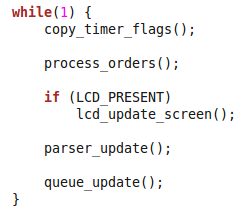
\includegraphics{pictures/main_loop_code.png}}
 \caption{\label{main_loop}Die Hauptschleife}
\end{figure}
\section{Debug}
Eigene Mechanismen zum Debugging sind genau dann sehr wichtig, wenn man nicht mit den
gewohnten Werkzeugen dies tun kann. Während der Laufzeit verstehen was in dem kleinen
Microcontroller vor sich geht ist essentiel, allerdings auch nicht sehr simpel, denn
die einzigen Möglichkeiten, die die Platine hat mit der Aussenwelt zu kommunizieren
beschränken sich auf 5 LED's, ein 4*20 Zeichen LCD, eine USART und eine I2C-Bus 
Schnittstelle. Der Aussagegehalt von den LED's (insbesondere da diese sich geweigert
haben zuverlässig zu funktionieren) und der LCD ist doch sehr begrenzt (man kann nicht
viele Informationen auf einem 4*20 Zeichen LCD unterbringen). Die Wahl fiel dann auf
die USART Schnittstelle, da der Arbeitscomputer, an dem das Debugging durchgeführt wurde
einen solchen Anschluss besitzt, aber über keinen I2C Anschluss verfügt.
Mithilfe der Debugausgaben kann man protokollieren, was das System in jedem
Schleifendurchlauf getan hat und dadurch das Verhalten analysieren, um schlussendlich
Fehler aufzuspüren. 
\section{Drive, Motor und PID}
Das Motor bindet zum einen das System an die Motoren und an die anderen nötigen
Fahrelemente an, wohingegen das Drive Modul die Services, die das Motor Modul anbietet
abstrahiert und in einer weise Zusammenfasst, die es dem System erlaubt auf sehr einfache
Art und Weise die Motoren zu bedienen.
Das PID Modul, welches größtenteils aus der vorhergegangen Studienarbeit übernommen wurde
\cite{STUD_TIMO}, ist für den Fehlerausgleich der Radbewegungen zuständig. Genauer: Es
errechnet die korrigierten Werte für die Räder, die dann vom Drive Modul an diese auch
weiter geleitet werden. Die Fehler die auftreten können sind vielfältig und nicht besonders
groß, wie zum Beispiel eine kleine Varianz in der Geschwindigkeit eines Rades oder ähnliches.
Damit aber das Fahrverhalten stabiler wird müssen diese Fehler korrigiert werden.
\section{IO, I2C und USART}
Das IO Modul stellt für das System einheitliche Funktionen zur Verfügung um Daten zu lesen als
auch zu schreiben. Hierbei kann es dem Benutzer der Funktionen egal sein, welche Schnittstelle
letztendlich für die Kommunikation genutzt wird. Das IO Modul kümmert sich um die Unterschiede
zwischen USART und I2C.
Sowohl das I2C als auch das USART Modul kümmern sich hauptsächlich um das Initialisieren der
Hardware und das behandeln der Interrupt Service Routinen.
\section{Order und Queue}
Das Order Modul ist das größte aller Module. Es beinhaltet zum einen den Typ, mit dem Befehle
intern dargestellt und verarbeitet werden. Aufbauend auf den Typ, dem einige unterstützende
Funktionen zugeteilt sind um wiederkehrende Aufgaben zu erleichtern, existiert im Order
Modul auch die Order Funktionen. Diese Order Funktionen sind Handler-Funktionen für die
im Protokoll spezifizierten Befehle. Falls ein Befehl länger benötigt, bis er als beendet
gelten kann, wird die entsprechende Order Funktion mit dem korrespondierenden Befehl in jeder
Iteration der Hauptschleife aufgerufen. Diese kann dann eventuell Wartungsarbeiten an dem
Befehl durchführen und überprüfen, ob dieser beendet ist und entsprechend seinen Status ändern.
Durch diesen Aufbau ist eine Hauptschleifeniteration sehr kurz, aber auch komplizierte Befehle
oder solche deren Parameter und Durchführung überwacht werden müssen sind hierdurch möglich.\\
Durch das Queue Modul ist es möglich der Motorplatine mehrere Befehle direkt hintereinander
zu übermitteln, die dann einer nach dem anderen ausgeführt werden, außerdem kümmert die
Queue sich darum, das Prioritäts-Befehle nicht eingereiht werden sondern bei der nächsten
Hauptschleifeniteration ausgeführt werden.
\section{Timer, Parser und Options}
Diese drei Module haben hauptsächlich eine unterstützende Funktion, so bringt das Timer Modul
die Möglichkeit mit in bestimmten zeitlichen Intervallen Befehle auszuführen. Der Parser
fasst einzelne Bytes logisch zu Befehlen zusammen und übergibt diese der Queue. Das Options
Modul beinhaltet die Einstellungen, die das Verhalten des gesamten Systems beeinflussen, wie
z.B. ob Debugging Ausgaben aktiviert sind, mit was für einer Geschwindigkeit das ABS bremst
und einiges mehr.

\cleardoublepage

\chapter{Protokoll\label{chapter_protokoll}}
Die Praktikumsplatine muss mit der Motorplatine kommunizieren, um das Fahrzeug in Bewegung zu setzen.
Diese Kommunikation sollte möglichst
effizient erfolgen. Die Entwicklung eines guten Protokolls ist deshalb
sehr wichtig für das gesamte System.\\
Das Vorläufer-Protokoll benutzte Zeichenketten, um Instruktionen zu übermitteln.
Dies hat zwei gravierende Nachteile. 
Zum einen nimmt das Zusammensetzen der Zeichenketten mithilfe der verfügbaren Prozessoren
sehr viel Rechenleistung in Anspruch.
Zum anderen ist durch die Verwendung der Zeichenketten die Informationsdichte der Instruktionen
nicht sehr hoch, und es fällt zusätzliche Wartezeit bei der Übermittlung an.

\section{Grundlegende Konzepte}
Da die Kommunikations-Einrichtungen der Hardware Byte-orientiert sind, wurde das
Protokoll ebenfalls Byte-orientiert aufgebaut. Im Gegensatz zu dem Vorgänger-Protokoll
werden also keine Zeichenketten benutzt, um die Informationen zu repräsentieren, sondern
nur der Wert der einzelnen Bytes.\\
Ein Befehl ist eine Folge von n Bytes, wobei n mindestens 1 und maximal der im Code
eingestellten Größe der Befehlsstruktur entspricht. 
Die maximale Länge der einzelnen eingebauten Befehle beträgt 9 Bytes.
Das erste Byte eines Befehls hat eine
besondere Bedeutung. Dieses Byte wird Kommando-Byte genannt. Das Kommando-Byte
ist in zwei Teile geteilt. Der erste Teil umfasst die 4 Bits mit der niedrigsten Wertigkeit und
wird Befehlscode genannt. Der Befehlscode spezifiziert die Art des Befehls.
Der zweite Teil beinhaltet die höchstwertigen 4 Bits. Darin werden Optionen
gesetzt, die den im Befehlscode angegebenen Befehl modifizieren. Die Kombination
von Befehlscode und Optionen legt auch die Länge des Befehls fest. Alle dem
Kommando-Byte folgende Bytes sind Parameter, wie z.B. die Geschwindigkeit der Räder.\\
Da 4 Bits für Befehlscodes zur Verfügung stehen, sind 16 verschiedene Befehle möglich.
Sechs Befehle wurden im Zuge dieser Arbeit implementiert; das würde noch Platz für
10 weitere Befehle lassen. Das Protokoll sollte allerdings noch mehr Freiheiten
für zukünftige Erweiterungen bieten, deswegen wurde einer der Befehlscodes
reserviert. Dieser reservierte Befehlscode und dessen Behandlung im Code ermöglichen
es, dass es mehr als ein Kommando-Byte geben kann. Damit ist es möglich, Befehle einfach 
hinzuzufügen, die nicht in das Schema ''ein Kommando-Byte, viele Parameter'' passen.\\
Wenn Parameter übertragen werden müssen, die mehr als ein Byte benötigen, wird zuerst
das höchstwertige Byte übertragen. Danach, absteigend nach der Wertigkeit, folgen die anderen
Bytes.\\
Durch die volle Ausnutzung der Bytes gibt es kein Protokoll-spezifisches STOP- oder START-Byte.
Das bedeutet, dass das Protokoll sich auf die Flusskontrolle der zugrunde liegenden Hardware
verlässt.

\section{Eingebaute Befehle}
Sechs Befehle und die Infrastruktur für den reservierten Befehlscode wurden implementiert.
Im Nachfolgenden werden die Befehle einzeln vorgestellt. Dabei wurde der Befehlscode bei
jedem Befehl in hexadezimaler Schreibweise als ganzes Byte dargestellt.

\subsection{Extended-Instruction - 0x00}
Dieser Befehl ist ein Platzhalter für zukünftige Befehle, die mehr als ein Kommando-Byte benötigen,
oder für den Fall, dass alle normalen Befehlscodes bereits vergeben sind. Der Befehlscode ist \textbf{0x00}.\\
Im Code werden solche Befehle mit besonderen Funktionen behandelt. Die 
parser\_\-extended\_\-order\_\-complete-Funktion ist ein Beispiel hierfür. Diese
besonderen Funktionsvarianten gibt es allerdings nur im Parser.
Nach dem Verlassen des Parsers wird eine Extended-Instruction wie ein normaler Befehl behandelt.
Die zusätzlichen Funktionen waren nötig, weil sich diese Befehle im Aufbau von normalen Befehlen stark unterscheiden.

\subsection{Control - 0x01}
Mit diesem Befehl kann das System gesteuert werden. Darunter fallen Aufgaben wie das
Reseten des gesamten Programms, das Anhalten der Befehlsausführung, und die Manipulation
der Befehls-Warteschlange. Der Befehlscode für diesen Befehl ist \textbf{0x01}. Außerdem ist der Control-Befehl
ein priorisierter Befehl, d.h. er wird bei dem nächsten Hauptschleifendurchlauf ausgeführt und nicht
an die Warteschlange angereiht.\\
Die in Tabelle \ref{protocol_control} beschriebene Bitmaske wird mit dem Befehlscode verodert
und ergibt das Kommando-Byte. Bei manchen Befehlen können mehrere Optionen zur gleichen Zeit
gewählt werden; dies ist hier nicht der Fall. Die Optionen dieses Befehls schließen sich
gegenseitig aus. Die Länge der Befehle mit vorgenanntem Befehlscode beläuft sich auf 1 Byte, sodass
 nur das Kommando-Byte gesendet werden muss.
\begin{table}[htb]
\begin{center}
	\begin{tabularx}{\linewidth}{|l|c|c|X|}
		\hline
		\textbf{Option} & \textbf{Bitmaske} & \textbf{resultierendes} & \textbf{Beschreibung} \\
		                &                   & \textbf{Kommando-Byte}   & \\
		\hline
		\hline
		Reset 			& 0x10 				& 0x11                    & Hardware-Reset \\
		\hline
		Stop Queue		& 0x20				& 0x21                    & Der Aktuelle Befehl wird verworfen. Die Warteschlange wird angehalten, aber nicht verworfen. \\
		\hline
		Continue Queue	& 0x30				& 0x31                    & Der nächste Befehl in der Warteschlange wird ausgeführt. \\
		\hline
		Clear Queue		& 0x40				& 0x41                    & Die Warteschlange wird gelöscht. \\
		\hline
		Stop Drive		& 0x50				& 0x51                    &Befehl wird angehalten, Fahrzeug geht zum aktiven Bremsen über. \\
		\hline
	\end{tabularx}
	\caption{\label{protocol_control} Optionen des Control-Befehls}
\end{center}
\end{table}

\subsection{Query - 0x02}
Manchmal ist es wichtig, dass die kontrollierende Praktikumsplatine verschiedene Laufzeitwerte
der Motorplatine kennt. Dieser Befehl, dem der Befehlscode \textbf{0x02} zugeordnet ist, ermöglicht
es, die Geschwindigkeit der Räder, die Anzahl der Befehle in der Warteschlange und den aktuellen
Befehl abzufragen. Die Optionen schließen sich gegenseitig aus, und die Länge des Befehls beträgt
immer 1 Byte. Der Befehl ist wie der Control-Befehl ein priorisierter Befehl. Er wird also
nicht an die Warteschlange angereiht.\\
Wenn nach Senden dieses Befehls an die Motorplatine kurz darauf versucht wird, über den I2C-Bus
das Ergebnis zu lesen, kann der Fall eintreten, dass es noch nicht vorliegt.
Das geschieht besonders dann, wenn der aktuelle Befehl angefordert wurde.
In diesem Fall muss die Lese-Operation nochmals gestartet werden.\\
Die Länge des aktuellen Befehls muss mit übertragen werden, damit die Praktikumsplatine
diesen Befehl, den die Motorplatine zurückgibt, auch verwerten kann.
Es ist deshalb nötig, dass die Praktikumsplatine zwei Lese-Operationen durchführt,
wobei die erste eine Länge von einem Byte hat und außerdem spezifiziert, wie lang die zweite Antwort in Bytes ist.

\begin{table}[htb]
\begin{center}
	\begin{tabularx}{\linewidth}{|c|c|X|l|}
		\hline
		\textbf{Bitmaske} & \textbf{resultierendes} & \textbf{Beschreibung} & \textbf{Antwortlänge} \\
		                  & \textbf{Kommando-Byte}  &                       & \textbf{in Bytes}\\
		\hline
		\hline
		0x10              & 0x12                    & Geschwindigkeit des linken Rades & 1 \\
		\hline
		0x20              & 0x22                    & Geschwindigkeit des rechten Rades & 1 \\
		\hline
		0x30              & 0x32                    & Anzahl der Befehle in der Warteschlange & 1 \\
		\hline
		0x40              & 0x42                    & Aktueller Befehl & 2 - 16 \\
		\hline
	\end{tabularx}
	\caption{\label{protocol_queue} Optionen des Query-Befehls}
\end{center}
\end{table}

\subsection{Drive - 0x03}
Der am häufigsten benutzte Befehl ist der Drive-Befehl. Durch ihn werden die Räder des Fahrzeugs
in Bewegung gesetzt. Ihm ist der Befehlscode \textbf{0x03} zugeteilt, und seine Länge beträgt zwischen 3
und 7 Bytes. Im Minimalfall besteht der Befehl aus dem Kommando-Byte und je einem Byte für
die gewünschte Geschwindigkeit der einzelnen Räder. Ohne die Angabe einer Abbruchbedingung für
beide Räder würde dieser Befehl endlos laufen, oder solange, bis mithilfe des Control-Befehls
die Ausführung unterbrochen wird. Die Abbruchbedingungen werden Trigger genannt. 
Die Räder sind mit zwei Trigger-Arten ausgerüstet:
Die Positions-Trigger und die Zeit-Trigger. Die Positions-Trigger stoppen
das Rad, dem sie zugeordnet wurden, nachdem eine bestimmte Anzahl an Interrupts von dem Rad
ausgelöst wurden. Die Zeit-Trigger stoppen das Rad, nachdem die angegebene Fahrzeit erreicht
wurde. 
Dadurch kann jedes Rad für sich entweder durch keinen Trigger, durch einen Zeit-Trigger
oder durch einen Positions-Trigger beeinflusst werden.
Triggerwerte sind
2 Bytes lang und nur positiv. Die Geschwindigkeit ist 1 Byte lang und kann auch negativ sein.
Dem Kommando-Byte folgt daher das Byte für die Geschwindigkeit des linken Rades, dann
das Byte für die Geschwindigkeit des rechten. Falls Triggerwerte angegeben werden müssen,
erfolgt dies nach den Geschwindigkeitsangaben.
Man beginnt ebenfalls mit dem Triggerwert für das linke Rad, dann folgt der
Wert für das rechte.\\
Zusätzlich zu diesen Fahrmöglichkeiten gibt es einen speziellen Fahrmodus, der für
die ''Geradeaus-Fahrt'' optimiert ist. Er wird als ''Fahrt mit Differenzausgleich''
bezeichnet. Hierbei wird versucht, die Differenz beider Räder möglichst auf 0 zu
halten. Wegen der Geradeaus-Fahrt entfällt die zweite Geschwindigkeitsangabe, und 
die Bitmasken für die Trigger des rechten Rades gelten für beide Räder. Eine weitere
Bitmaske erlaubt es, den Startwert des Differenzwertes festzulegen. Dieser ist dann
der einzige Parameter, 2 Bytes lang und vorzeichenbehaftet.\\
Zur Konstruktion des Kommando-Bytes dieses Befehls wird der Befehlscode mit der Bitmaske
für das linke Rad und für das rechte Rad verodert. Es muss eine der drei Möglichkeiten
ausgewählt werden, die in dem oberen Teil der Tabelle \ref{protocol_drive} vorgestellt werden.
Dies gilt nur, wenn nicht die Bitmaske 0x30 oder 0xc0 verwendet wird.
\begin{table}[htb]
\begin{center}
	\begin{tabular}{c}
	\begin{tabularx}{\linewidth}{|p{2cm}|l|l|X|}
		\hline
		\textbf{Option} & \textbf{Bitmaske links} & \textbf{Bitmaske rechts} & \textbf{Beschreibung} \\
		\hline \hline
		Kein Trigger	& 0x00						   & 0x00						   & Endlosfahrt \\ \hline
		Zeit-Trigger	& 0x10						   & 0x40						   & zeitlich begrenzte Fahrt\\ \hline
		Positions-Trigger & 0x20					   & 0x80						   & fährt eine bestimmte Strecke \\ \hline
		Fahrt mit Differenz-Ausgleich & 0x30		   & -						   & beide Räder fahren mit derselben Geschwindigkeit geradeaus \\ \hline
		Differenz setzen & 0xc0					   	   & -						   & setzt die Differenz der Räder \\ \hline
	\end{tabularx}\\
	Optionen des Drive-Befehls
	\\
	\begin{tabularx}{\linewidth}{|l|l|l|X|}
		\hline
		\textbf{Byte-Anzahl} & \textbf{Option} & \textbf{Wertebereich} & \textbf{Beschreibung} \\
		\hline
		\hline
		1					 & - & -128 bis 127 & Geschwindigkeit des linken Rades \\
		\hline
		1					 & - & -128 bis 127 & Geschwindigkeit des rechten Rades\\
		\hline
		2					 & Zeit-Trigger & 0 bis 65535 &  die Fahrzeit des linken Rades (in 100 ms)\\
		\hline
		2					 & Positions-Trigger & 0 bis 65535 &  Anzahl der Ticks für die Fahrt des linken Rades\\
		\hline
		2					 & Zeit-Trigger & 0 bis 65535 &  die Fahrzeit des rechten Rades (in 100 ms)\\
		\hline
		2					 & Positions-Trigger & 0 bis 65535 &  Anzahl der Ticks für die Fahrt des rechten Rades\\
		\hline
	\end{tabularx}
	\end{tabular}
	\caption{\label{protocol_drive} Parameter des Drive-Befehls}
\end{center}
\end{table}

\subsection{Advanced-Drive - 0x04}
Der Advanced-Drive-Befehl, der den Befehlscode \textbf{0x04} besitzt, verhält sich grundsätzlich
wie der normale Drive-Befehl. Er bietet allerdings mehr Möglichkeiten für den Einsatz der Trigger.
Wird der Befehl ohne Trigger
verwendet, so ist er mit dem Drive-Befehl identisch. Werden diese jedoch verwendet,
müssen für jedes Rad zwei Trigger-Werte angegeben werden. Es werden also immer Zeit-
und Positions-Trigger verwendet. Je nach gewählter Option werden sie miteinander mit einem logischen
UND oder einem logischen ODER verknüpft. So ist es möglich, Fahrbefehle
zu erteilen, die entweder eine bestimmte Strecke oder eine bestimmte Zeit fahren.
\begin{table}[htb]
\begin{center}
	\begin{tabularx}{\linewidth}{|X|l|l|X|}
		\hline
		\textbf{Option} & \textbf{Bitmaske Links} & \textbf{Bitmaske Rechts} & \textbf{Beschreibung} \\
		\hline
		\hline
		Kein Trigger				& 0x00						   & 0x00						   & Endlosfahrt \\
		\hline
		Zeit-Trigger ODER Positions-Trigger	& 0x10						   & 0x40						   & Fahrt bis Erreichen eines Triggers\\
		\hline
		Zeit-Trigger UND Positions-Trigger  & 0x20						   & 0x80						   & Fahrt bis Erreichen beider Trigger\\
		\hline
	\end{tabularx}
	\caption{\label{protocol_advanced_drive} Optionen des Advanced-Drive-Befehls}
\end{center}
\end{table}

\subsection{SetPID - 0x05}
Das PID-Modul benutzt mehrere Parameter, um den Fehlerausgleich durchzuführen. Diesen
Parametern sind im Programmcode bereits Standardwerte zugewiesen worden. Es kann aber
vonnöten sein, diese Parameter anzupassen. Dafür ist der SetPID-Befehl erforderlich.
Dieser besitzt den Befehlscode \textbf{0x05}. Seine Länge beträgt immer 9 Bytes. Es müssen
alle Werte dem SetPID-Befehl übergeben werden. Jeder Wert benötigt 2 Bytes.
Die Werte können auch negativ sein. Sie werden in der Reihenfolge angegeben,
wie sie im oberen Teil der Tabelle \ref{protocol_setpid} zu finden sind.
Die genaue Auswirkung dieser Einstellungen sollte vom Benutzer in der Studienarbeit von
Timo Klingeberg \cite{STUD_TIMO} nachgelesen werden.
\begin{table}[htb]
\begin{center}
	\begin{tabular}{c}
	\begin{tabularx}{\linewidth}{|l|l|l|X|}
		\hline
		\textbf{Byte-Anzahl} & \textbf{Position} & \textbf{Wertebereich} & \textbf{Beschreibung} \\
		\hline
		\hline
		2					 & 1 & -32768 bis 32767 & \textbf{P}roportionaler Faktor\\
		\hline
		2					 & 2 & -32768 bis 32767 & \textbf{I}ntegraler Faktor\\
		\hline
		2					 & 3 & -32768 bis 32767 & \textbf{D}ifferentieller Faktor\\
		\hline
		2					 & 4 & -32768 bis 32767 & maximaler Fehlersummen-Modifikator\\
		\hline
	\end{tabularx}\\
	\\
	\begin{tabularx}{\linewidth}{|l|c|X|}
		\hline
		\textbf{Option} & \textbf{Bitmaske} & \textbf{resultierendes Kommando-Byte} \\
		\hline
		\hline
		linkes Rad	& 0x00 & 0x05 \\
		\hline
		rechtes Rad	& 0x10 & 0x15 \\
		\hline
		beide Räder & 0x20 & 0x25 \\
		\hline
	\end{tabularx}
	\end{tabular}
	\caption{\label{protocol_setpid} Optionen des SetPID-Befehls}
\end{center}
\end{table}

\subsection{Option - 0x06}
Der Option-Befehl besitzt den Befehlscode \textbf{0x06} und hat eine Länge von 2 Bytes.
Durch ihn können bestimmte Variablen auf der Motorplatine während der Laufzeit
geändert werden. Momentan kann damit das ABS (siehe Kapitel \ref{chapter_abs}) angepasst werden. Nach dem
Kommando-Byte folgt der neue Wert der Variablen.
\begin{table}[htb]
\begin{center}
	\begin{tabularx}{\linewidth}{|l|l|l|X|}
		\hline
		\textbf{Bitmaske} & \textbf{Default} & \textbf{Wertebereich (Bytes)} & \textbf{Beschreibung} \\
		\hline
		\hline
		0x10 & 40 & 1 bis 127 (1) & Geschwindigkeitswert beim aktiven Bremsen\\
		\hline
		0x20 & 1 & 0 oder 1 (1) & Schalter zum Aktivieren der aktiven Bremsung (eine 1 bedeutet die Aktivierung)\\
		\hline
		0x30 & 1 & 0 oder 1 (1) & Schalter zum Aktivieren der aktiven Bremsung \textbf{des} Rades, das seinen Trigger erreicht hat\\
		\hline
		0x40 & 1 & 0 oder 1 (1) & Schalter zum Aktivieren der aktiven Bremsung, wenn kein Befehl bearbeitet wird\\
		\hline
	\end{tabularx}
	\caption{\label{protocol_option} Optionen des Option-Befehls}
\end{center}
\end{table}

\cleardoublepage

\chapter{Implementierung der Betriebssoftware}
Die Betriebssoftware wurde, wie in der Aufgabenstellung festgelegt in C geschrieben.
Hierbei fiel die Wahl auf den Standard C99, der mit einigen sprachlichen
Aktualisierungen gegenüber C89 aufwarten kann. Als Compiler wurde eine Version der
GNU Compiler Collection (GCC) mit einem Backend für AVR-kompatiblen Assembler benutzt.
Außer der C Standard Library und der AVR IO Library besitzt die Software keine externen
Abhängigkeiten im Code.
\section{Die Hauptschleife}
Die Hauptschleife ist in dieser Implementierung eine Endlosschleife, da die Beendigung dieser
Schleife dazu führen würde, dass das System nicht mehr reagiert.
Wie in Abb. \ref{main_loop} zu sehen ist, werden in der Hauptschleife vier wichtige Funktionen
aufgerufen.
\subsection{process\_orders()}
Die process\_\-orders()\--Funktion bearbeitet die Befehle, die bereits in der Queue sind. Dafür holt
sich die Funktion den aktuellen Befehl von der Queue. Falls es solch einen Befehl gibt ruft die
Funktion eine Verteilerfunktion auf. Diese wiederum ruft die zugehörige Befehlsfunktion auf, indem
die untersten vier Bits des ersten Befehlsbytes als Index für eine Call-Table benutzt werden (siehe
Abb. \ref{dispatch_function}).\\
\begin{figure}[htb]
 \centering
 \scalebox{0.6}{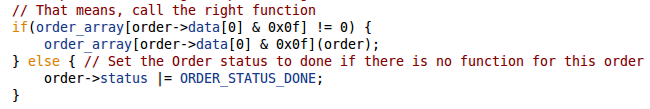
\includegraphics{pictures/dispatch_function.png}}
 \caption{\label{dispatch_function}Die Verteilerfunktion}
\end{figure}
Falls kein Befehl vorliegt oder die Queue angehalten wurde, ruft die process\_\-orders()-Funktion die
Funktion zum aktiven Bremsen auf. Das aktive Bremsen wird in Kapitel \ref{chapter_abs} behandelt.
\subsection{lcd\_update\_screen()}
In dem Fall, dass ein LCD angeschlossen ist, können dort Informationen ausgegeben werden. Ob ein LCD
angeschlossen ist wird über die Stellung eines DIP-Schalters auf der Platine geregelt.\\
Da das synchrone Aktualisieren des LCD sehr viel Zeit benötigt (vgl. Kapitel \ref{chapter_lcd_problem}), wird
während dieser Funktion maximal ein Zeichen an das LCD geschickt. Dies wird erreicht indem das Busy-Flag,
welches signalisiert, dass das LCD noch beschäftigt ist, abgefragt wird. Falls es nicht gesetzt ist und
es noch Daten zum aktualisieren gibt, wird das nächste Zeichen an das LCD gesendet.\\
Auf dem LCD werden die Versionsnummer der Betriebssoftware, der Status einiger system-weiter Variablen und
der aktuelle ausgeführte Befehl angezeigt. Falls nun ein Befehl bearbeitet wird, der länger als einen
Schleifendurchlauf benötigt (das sind z.B. alle Fahr-Befehle), ruft die lcd\_\-update\_\-screen()-Funktion
die lcd\_\-update\_\-info()-Funktion auf, die diese Informationen in einem Puffer konstruiert. Nach und nach
gibt die lcd\_\-update\_\-screen()-Funktion den Inhalt dieses Puffer an das LCD weiter.\\
Befehle die innerhalb eines Hauptschleifendurchlaufs abgearbeitet sind werden nicht ausgegeben und
generieren auch keinen Aufruf von lcd\_\-update\_\-info(). Dies ist nötig, da diese Befehle zu schnell abgearbeitet
werden. Es können vier bis fünf dieser Befehle abgearbeitet werden, bevor das LCD auch nur einmal vollständig
aktualisiert werden kann.
\subsection{parser\_update()}
Der Parser ist dafür zuständig aus den Bytes, die über I2C oder UART gelesen werden, Befehle in Form von
order\_t-Strukturen zu erstellen. Die parser\_\-update()-Funktion fragt beim IO-Modul nach, wie viele Bytes
zum Abholen bereit stehen. Diese werden dann geholt und an die Funktion parser\_\-add\_\-byte() übergeben.\\
Diese parser\_\-add\_\-byte()-Funktion fügt das Byte an die korrekte Stelle im Puffer ein. Wenn ein Befehl
komplett ist, was mit der parser\_\-order\_\-complete()-Funktion überprüft wird, gilt der Befehl als fertig und
alle weiteren Bytes, die hinzugefügt werden, landen in einer neuen order\_t-Struktur.\\
Damit erkannt werden kann, wann ein Befehl zu ende ist benutzt die parser\_\-order\_\-complete()-Funktion
die bytes\_\-needed()-Funktion, in der fest codiert ist, welcher Befehlscode mit welchen Optionen wie viele
Bytes benötigt. Dies ist auch eine der Stellen, die angepasst werden müssen, wenn ein neuer Befehl hinzugefügt
wird, oder bestehende verändert werden.
\subsection{queue\_update()\label{chapter_queue_update}}
Diese Funktion führt Wartungsarbeiten an der Befehlswarteschlange (Queue) durch. Dies beinhaltet neue
Befehle beim Parser-Modul abzuholen und diese korrekt einzureihen. Es gibt zwei Möglichkeiten, wie die Queue
diese neuen Befehle einreihen kann. Zum einen als normale Befehle, diese werden einer nach dem anderen abgearbeitet,
zum anderen als priorisierte Befehl. Es kann nur ein priorisierter Befehl in der Queue sein. Diese Befehle werden
umgehend in der nächsten Haupt\-schleifen\-iteration ausgeführt. In die Kategorie der priorisierten Befehle fallen
alle Queue-Kontroll-Befehle, wie z.B. pausieren, löschen, aktuellen Befehl verwerfen, etc. (vgl. Kapitel \ref{chapter_protokoll}).
\section{Das Aktive Brems-System (ABS)\label{chapter_abs}}
Das aktive Bremssystem bewirkt, dass die Räder versuchen ihre Position nicht zu verlassen. Dies wird realisiert indem
eine Referenz-Position für jedes Rad gespeichert wird. Während der Hauptschleife wird nun die tatsächliche Position mit
der Referenz-Position verglichen. In dem Fall, dass diese Positionen nicht übereinstimmen, werden die Motoren mit einer
einstellbaren Geschwindigkeit betrieben, um die Räder wieder auf die Referenz-Position zu bringen.\\
Die Referenz-Positionen werden an drei verschiedenen Stellen im Code gesetzt. Zum einen in der process\_\-orders()-Funktion
in der Hauptschleife, wenn der aktuelle Befehl beendet wurde, zum anderen in den Fahr-Befehls-Funktionen, falls ein Rad
früher als das andere seine Stopp-Bedingung erreicht hat.\\
Das ABS kann vom Benutzer während das System läuft, angepasst werden. So kann man die Geschwindigkeit ändern, mit der
die Motoren die Positions-Differenz ausgleichen. Außerdem kann man Teile des ABS deaktivieren oder auch wieder reaktivieren
sowie das gesamte ABS abschalten, bzw. wieder anschalten. Damit kann der Benutzer das ABS an seine Wünsche anpassen.
\section{Befehle: Struktur und Funktionen}
Die Struktur (Abb. \ref{order_type}), die einen Befehl im System repräsentiert, besteht hauptsächlich aus einem Array, in dem die eigentlichen Daten
gespeichert sind, und einem Status-Byte, in dem Statusinformationen in Form von Flags gespeichert werden.
\begin{figure}[htb]
 \centering
 \scalebox{0.6}{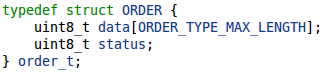
\includegraphics{pictures/order_t.png}}
 \caption{\label{order_type}Befehlsstruktur}
\end{figure}
Das erste Byte dieses Arrays ist das Typ-Byte, das die Art des Befehls und die zugehörigen Optionen spezifiziert. Der
Befehlscode (die unteren vier Bits des Typ-Bytes) 0 ist für zukünftige Erweiterungen Reserviert, die mehr als ein Typ-Byte
benötigen. Des weiteren sind die Befehlscodes 1 bis 6 durch diese Arbeit bereits definiert und mit Funktionalität erfüllt.
Die Befehlscodes 7 bis 15 sind noch nicht definiert und können für zukünftige Erweiterungen benutzt werden, die mit einem
Typ-Byte auskommen.\\
Alle auf das Typ-Byte (oder die Typ-Bytes im Falle des Befehlscodes 0) folgenden Bytes sind Parameter. Die Anzahl und Länge
dieser hängt von der Spezifikation des Befehls ab. Grundsätzlich gilt aber, dass bei Parametern, mit mehr als ein Byte Länge,
zuerst das höchstwertige Byte im Array gespeichert wird, dann absteigend bis zum niederwertigsten Byte.\\
Oft benutze Aktionen bezüglich der Befehlsstruktur wurden zusammengefasst (siehe Abb. \ref{order_init} und \ref{order_copy}).
Vor der Untersuchung des Laufzeitverhaltens und der damit einhergehenden Optimierungen, wurden diese beiden Funktionen
durch for-Schleifen implementiert, was sich aber als langsamer als die Standard C Funktionen memset() und memcpy()
herausstellte.
\begin{figure}[htb]
 \centering
 \scalebox{0.6}{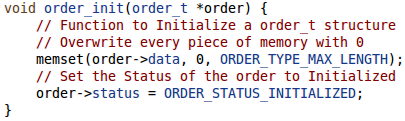
\includegraphics{pictures/order_init.png}}
 \caption{\label{order_init}order\_init()-Funktion}
\end{figure}
\begin{figure}[htb]
 \centering
 \scalebox{0.6}{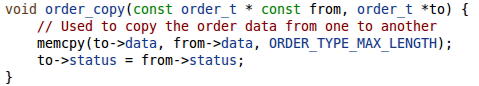
\includegraphics{pictures/order_copy.png}}
 \caption{\label{order_copy}order\_copy()-Funktion}
\end{figure}
\section{Datenpfad von Befehlen}
Befehle werden entweder über die UART oder die I2C Schnittstelle byteweise empfangen. Diese Schnittstellen werden über
Interrupt Service Routinen bearbeitet, um zeitnah auf eingehende Daten zu reagieren, da diese Übertragung die größte
Latenz-Quelle darstellt (I2C: ca. 270 \textmu{}s pro Byte; UART: ca 139 /textmu{}s pro Byte). In diesen Interrupt Service Routinen wird
das empfangene Byte in den Eingangspuffer gelegt. Wenn die Hauptschleife wieder die parser\_\-update()-Funktion erreicht,
wird die bisher empfangene Bytes abgeholt und in der Parser-Puffer abgelegt, um aus den Bytes order\_t Struktur Instanzen
zu generieren. Wenn der Befehl fertig im Parser vorliegt, ruft ihn queue\_\-update() ab und reiht ihn in die Warteschlange
ein (siehe Kapitel \ref{chapter_queue_update}). Von der Warteschlange holt sich die process\_\-orders()-Funktion den
aktuellen Befehl und führt die zugeordnete order\_function-Funktion solange aus, bis im Status-Byte (vgl. Abb. \ref{order_type})
das ORDER\_\-STATUS\_\-DONE Flag gesetzt wurde und entfernt diese dann aus der Warteschlange.\\
Falls der Befehl, der bearbeitet wird, eine Ausgabe von Daten bewirkt, wird in der entsprechenden order\_\-function-Funktion
die auszugebenden Daten in den Ausgabepuffer des IO-Framework angereiht. Dieses Framework wird dann, sobald möglich, diese Daten
über die ausgewählte Schnittstelle senden (bei UART wird sofort angefangen zu senden, bei I2C muss gewartet werden, bis die Daten
vom Benutzer abgerufen werden).
% Datenpfadbild
\section{Debug-Ausgaben \label{impl_debug}}
Das Problem mit Debug-Ausgaben ist, dass sie notwendig sind, insbesondere wenn die Benutzung eines üblichen Debuggers nicht
ohne weiteres möglich ist. Debug-Ausgaben benötigen entsprechenden Code, nicht nur um die Ausgaben überhaupt zu ermöglichen,
sonder auch an vielen Stellen im Code, um wirklich etwas zu bestimmten Zeitpunkten auszugeben. Diese Ausgaben, selbst wenn
sie nicht gemacht werden müssen, indem sie mit if-Statements umschlossen werden (siehe Abb. \ref{debug_trick}), verlangsamen
das gesamte System. Während der normalen Operation der Betriebssoftware im Praktikum, sind diese Ausgaben nicht nötig und für
die meisten Teilnehmer des Praktikums, nicht informativ. Damit die Ausgaben zum Zweck der Fehlerbehebung benutzt werden können,
muss der Benutzer eine entsprechende Kenntnisse des Codes vorweisen.\\
Aufgrund dieser fragwürdigen Hilfe, die diese Ausgaben einem durchschnittlichen Praktikanten bieten, und der negativen Auswirkung
der Ausgaben auf die Performance des Systems, wurde eine Prä-Prozessor Technik angewandt, die zusammen mit der eingestellten Stufe
der Code-Optimierung des Compilers diese beiden Probleme löst. Durch diese Technik werden die Debug-Ausgaben nur dann mitkompiliert,
wenn dem Compiler der Parameter -DDEBUG übergeben wird. Selbst dann ist es noch möglich mit einem DIP-Schalter auf der Platine
die Ausgaben auszuschalten, dann hat man aber immer noch die leichten negativen Auswirkungen auf die Performance. Normalerweise
wird die Betriebssoftware ohne diesen Parameter kompiliert. Das bedeutet, dass die Software neukompiliert werden muss, wenn
diese Debug-Ausgaben erwünscht sind.
\begin{figure}[htb]
 \centering
 \scalebox{0.5}{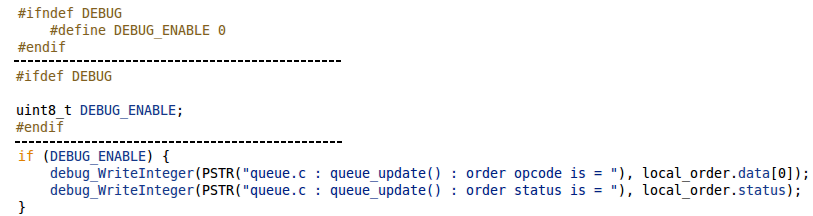
\includegraphics{pictures/debug_trick.png}}
 \caption{\label{debug_trick}Debug-Defines und die Verwendung im Code}
\end{figure}
\section{IO-Framework}
Das Ziel des IO-Frameworks war die Abstraktion der Ein- und Ausgabe von Daten von den zu Grunde liegenden Schnittstellen.
Die UART und die I2C Schnittstelle sind in der Benutzung sehr unterschiedlich. Statt überall im Code wo E/A stattfindet
jeweils für beide Schnittstellen Code einzufügen, wurde das IO-Framework als Zwischenschicht entwickelt. Es verfügt über sowohl
über einen Ausgabe- als auch über einen Eingabepuffer. Diese sind jeweils auf 256 Bytes festgelegt. Durch diese Definition
konnte das normale "Uberlaufverhalten der 8-Bit-Variablen ausgenutzt werden, um Modulo-Operationen zu ersetzen, welche
ungerechtfertigt viel Zeit in Anspruch nehmen.\\
Eine Besonderheit ist die Objekt-basierte Ausgabe von Daten. Ein Objekt hat mindestens ein Byte und maximal 256 Byte. Objekte
werden bei entweder komplett Übertragen oder gar nicht. Wenn ein Objekt nicht komplett übertragen werden konnte, wird bei der
nächsten Übertragen vom Anfang der Objektes wieder angefangen. Außerdem bewirkt die Ausgabe von Objekten bei Benutzung der I2C 
Schnittstelle, dass für jede Lese-Operation, die von der Praktikumsplatine eingeleitet wird, ein Objekt übermittelt wird.\\
E/A-Operationen geschehen nicht-blockend und gepuffert. Damit verbraucht die E/A nur Prozessor-zeit, wenn es nötig ist und
verschwendet diese nicht mit aktiven Warten.
\section{Unterstützende Bibliothek für die Praktikumsplatine}

\cleardoublepage

\chapter{Untersuchung des Laufzeitverhaltens}
Die Untersuchung der Laufzeitverhaltens wurde mithilfe eines Logik-
Analysers durchgeführt. Ein Logikanalyser misst wie lange und wann
ein Pin 1 und/oder 0 ist. Die Pins, die nötig sind um diese Messungen
durchzuführen, dürfen noch nicht belegt sein. Vorteilhafterweise
besitzt die Platine zwei Ports, die noch nicht belegt sind aber
trotzdem nach draußen gelegt wurden, somit konnte der Logik-
Analyser an die Platine angeschlossen und ein kleines Modul
geschrieben werden, um diese Pins setzen und wieder löschen zu
können. Diese Operationen wurden als Makros implementiert um den
Messungsoverhead so gering wie möglich zu halten.
\begin{center}
	\begin{tabular}{|c||c|c|}
		\hline
		\textbf{Makro} & \textbf{benötigte Takte} & \textbf{benötigte Zeit bei 16 MHz} \\ \hline \hline
		pin\_set() & 2 & 125 ns \\ \hline
		pin\_clear() & 2 & 125 ns \\ \hline
		pin\_toggle() & 4 & 250 ns \\ \hline
	\end{tabular}
\end{center}
Wie hier beschrieben sind die Zeiten für das Ausführen der Instruktion
zum setzen, löschen und umschalten von einzelnen Pins ziemlich gering.
Doch bei den Messungen insbesondere mit einem Leistungsfähigen und
sehr genauen Oszilloskop konnte herausgefunden werden, dass das eigentliche
wechsel des Stroms am Pin verhältnissmäßig langsam durchgeführt wird,
insbesondere das Abfallen des Stromes, also bei einer fallenden Flanke
benötigt ungefähr 2 us von denen allerdings, und hier liegt das Problem,
zwischen 0.5 und 1 us fälschlicherweise als \"high\" gemessen wird.
D.h. der Logikanalyser misst eine gewisse Zeitspanne einen \"falschen\" Wert.
(Er ist nicht physikalisch falsch nur logisch). Denn wenn der Strom abfällt
ist der bin schon nicht mehr gesetzt, der Logikanalyser allerdings betrachtet
dies teilweise immernoch als gesetzt.
Aufgrund dieses Umstandes als auch der Tatsache, dass das System nicht untersucht
werden kann ohne einen geringen Fußabdruck zu hinterlassen, sind die Messungen mit
einem abschätzbaren aber nicht genau vorhersagbaren Fehler im Vergleich zur
Wirklichkeit behaftet.

\cleardoublepage

\chapter{Zusammenfassung und Ausblick}
Das Ergebnis dieser Arbeit ist, dass die Platine auf Befehle schnell und korrekt reagiert,
solange diese nicht gravierend von den Spezifikation abweichen. Es gehen keine Interrupts verloren, und die
Platine reagiert auf Änderungen in Bruchteilen einer Sekunde.\\
Dennoch gibt es einige Punkte, die aufgrund der begrenzten Zeit nicht getestet oder implementiert
werden konnten.\\
So ist beispielsweise das Verhalten des ABS abhängig von der Dauer der Hauptschleife. Normalerweise
ist dies kein Problem. Wenn allerdings Debug-Ausgaben vorgenommen werden, kann das ABS sich
auf eine Art und Weise verhalten, die nicht erwünscht ist (dauerndes hin und her schwenken der Räder,
da kein Schleifendurchlauf während des Nullpunktes stattfindet). Um dies zu verhindern, kann man
einen Timer-Interrupt mit einer möglichst niedrigen Auflösung benutzen. Der Vorteil wäre hierbei,
dass das ABS nicht mehr abhängig von der Geschwindigkeit der Hauptschleife ist. Außerdem ist das
Abschalten des ABS gleichzusetzen mit dem Abschalten des zugehörigen Interrupts. Dieses wiederum
eliminiert den Overhead des ABS komplett, wenn es abgeschaltet ist. Dieser Overhead wird auf
ungefähr 2,5 \textmu{}s pro Schleifendurchlauf geschätzt. Der Nachteil besteht in einem geringen
Mehraufwand, da ein Funktionsaufruf durch eine Interrupt-Service-Routine ersetzt wird.\\
Eine weitere Erweiterungsmöglichkeit für das System besteht in erhöhter Robustheit und erweiterter
Fehlererkennung. So ist es möglich eintreffende Befehle auf komplette syntaktische Korrektheit
zu überprüfen und nur solche Befehle zu akzeptieren, die diese Tests bestehen. Diese Erweiterung
muss allerdings möglichst effizient und einfach erweiterbar implementiert werden, um zum einen nicht
entgegen der Designprinzipien des Systems zu handeln, als auch das Laufzeitverhalten nicht
schwerwiegend zu beeinträchtigen. Zusätzlich zu dieser Fehlererkennung kann die Robustheit des Systems
durch ein Überwachungssystem erhöht werden, welches in periodischen Abständen, ermöglicht durch
die eingebauten Timer, die einzelnen Module des Gesamtsystems auf Anzeichen von Problemen untersucht,
wie z.B. volle Puffer, runaway Befehle, Parser Status Korruption und dergleichen. Um die Möglichkeit
von runaway Code auszuschließen, ist die Benutzung des eingebauten Watchdog-Timers möglich, dessen
timeout Wert allerdings sehr sorgfältig gewählt werden muss. Der timeout Wert darf nicht kleiner sein
als die längste Hauptschleifen Iteration plus ein entsprechendes Sicherheitspolster.\\
Ein Bereich, der während der Arbeit vollkommen vernachlässigt wurde, ist die Möglichkeit die
Motorplatine in einen Idle-Modus zu schicken, in diesem Modus verbraucht wie Platine wesentlich weniger
Strom. Dies würde die Zeit verlängern, die eine Batterie an solch einem Fahrzeug hält, während die
Praktikanten an ihm arbeiten und die Motorplatine längere Zeit nichts zu tun hat. In dieser Hinsicht
wäre es auch interessant den Idle-Modus bzw. das Verhalten um dem Idle-Modus durch Befehle während der
Laufzeit steuern zu können.\\
Wie im Kapitel über die Laufzeituntersuchung beschrieben ist die Datenrate über den I2C-Bus der größte
limitierende Faktor bei der Übermittlung von Fahrbefehlen von der Praktikumsplatine an die
Motorplatine. Damit dieses Problem minimiert wird kann man zum einen erwägen den I2C-Bus im ''high-speed''
Modus operieren zu lassen, oder eine eigene Punkt-zu-Punkt Kommunikation mithilfe der freien Ports auf der
Motorplatine zu realisieren. Solch ein Maßgeschneiderter Port mit einem eigens dafür entwickelten Protokoll
könnte die Latenz, die durch das Senden des Befehls entsteht, erheblich verringern.

\cleardoublepage

\addcontentsline{toc}{chapter}{Literaturverzeichnis}
\bibliographystyle{unsrt}
\bibliography{thesis}
\cleardoublepage

\begin{appendix}
\begin{figure}[htb]
 \centering
 \scalebox{0.3}{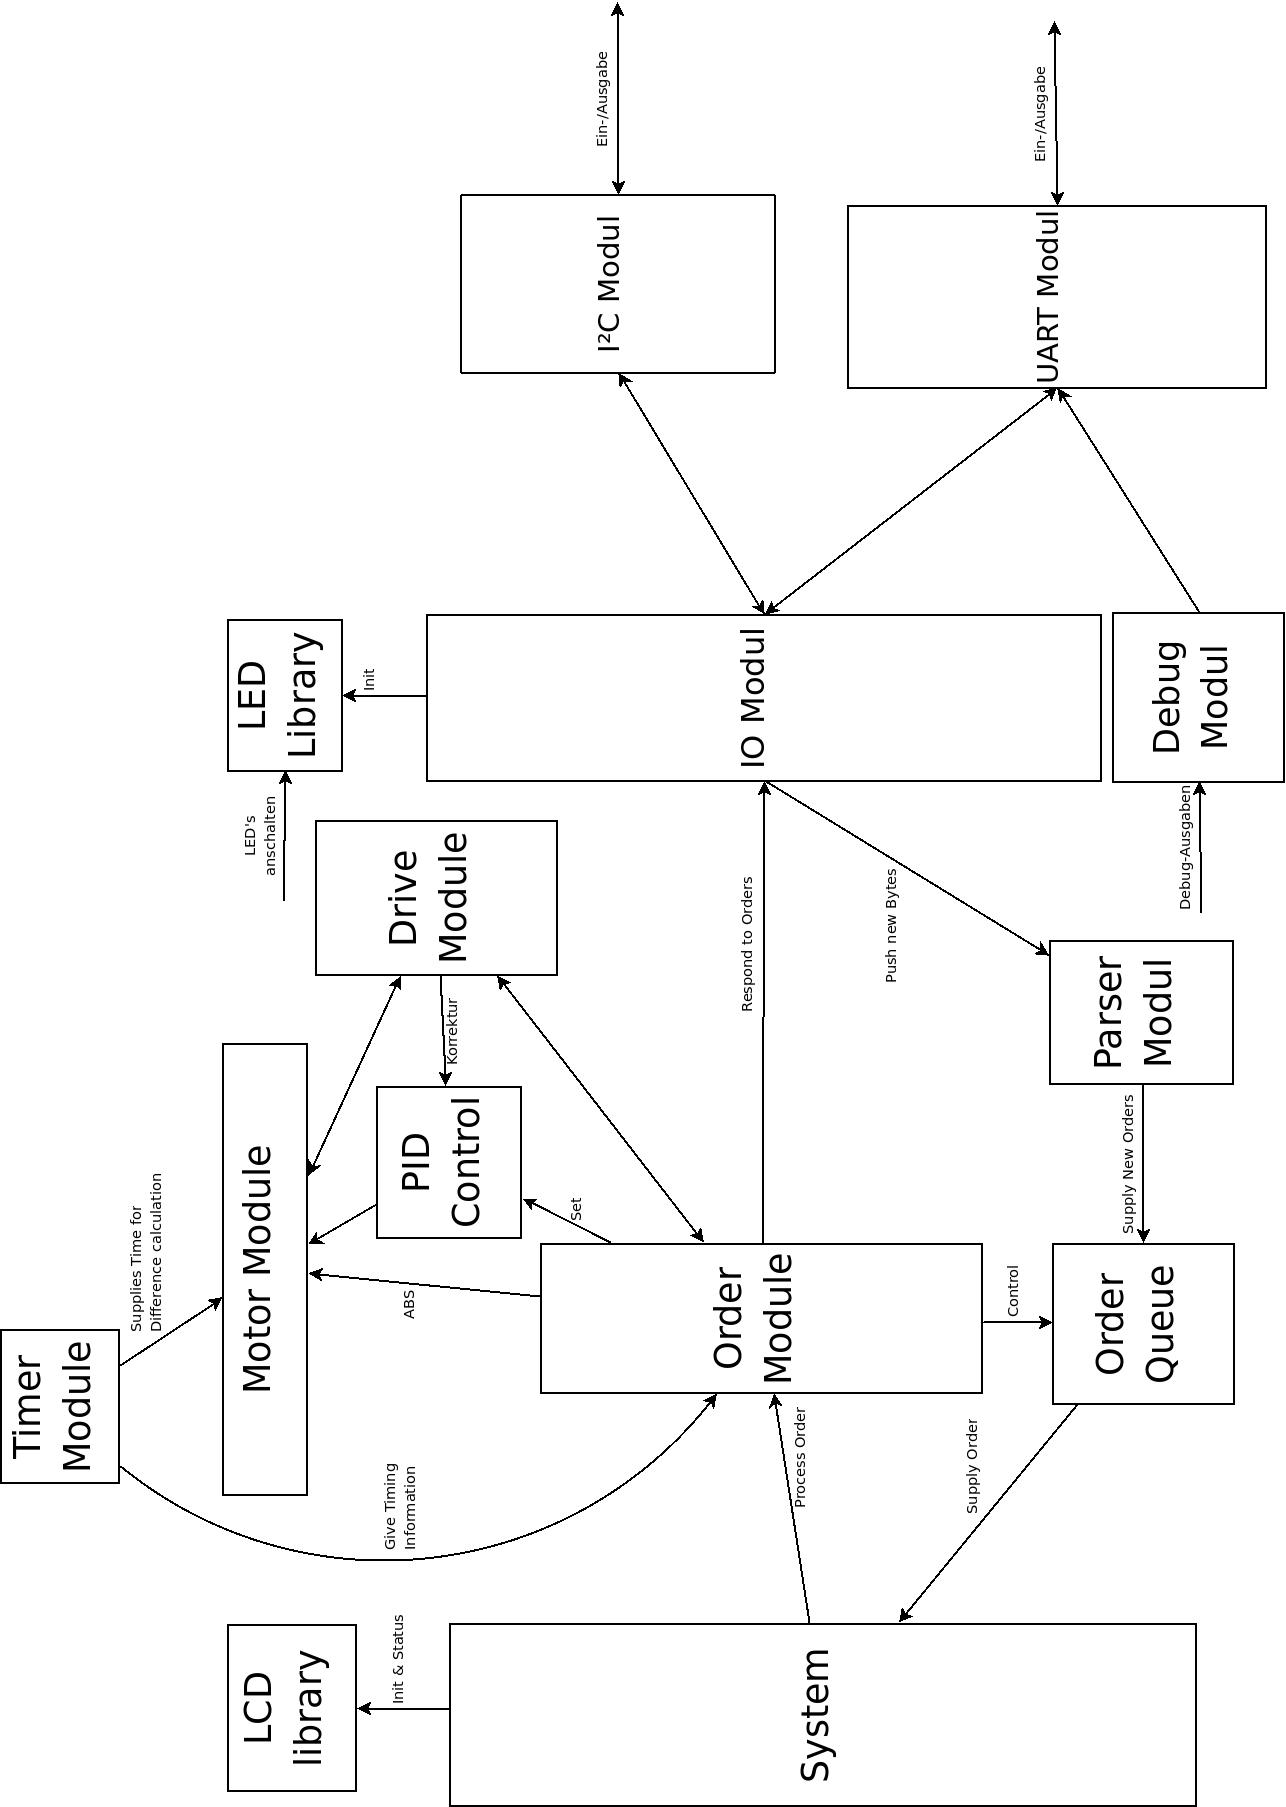
\includegraphics{pictures/modules.png}}
 \caption{\label{modules}Die Module und ihre Beziehungen}
\end{figure}

\cleardoublepage

\chapter{Inhalt der zugehörigen CD}
\begin{itemize}
	\item Der Quellcode der Betriebssoftware (inklusive Makefile).
	\item Die Quelldateien der vorliegenden Arbeit.
	\item Die vorliegende Arbeit im PDF.
	\item Die Quelldateien des Benutzerhandbuches.
	\item Das Benutzerhandbuch im PDF.
	\item Die Testreihen, die während der Optimierungsphase erstellt wurden.
	\item Die Programmcode-Dokumentation als doxygen-HTML-Dokumentation.
	\item Das Datenblatt des Mikrocontrollers.
	\item Das Benutzerhandbuch von Timo Klingeberg für die Motorplatine.
	\item Die Coding-Guidelines als Text-Datei.
\end{itemize}

\cleardoublepage

\chapter{Coding-Guidelines \label{appendix_cg}}
\begin{verbatim}
- Jede Einrückungsebene wird mit einem Tabulator eingerückt.
- Nach Kommentarzeichen folgt ein Leerzeichen.
- Geschweifte Klammern werden direkt nach dem entsprechenden
  Statement geöffnet.
Bsp.:
if (a < b) {
    // Do something
} else if (a > b) {
    // Do another thing
} else {
    // Whatever
}

- Funktionen werden nach folgendem Schema benannt:
    modul_namensteil1_..._namensteilN();
Bsp.:
    io_obj_start();

- Defines und globale Variablen (keine Datei-globale, nur
  System-globale) werden GROß geschrieben.
- Jede Funktion muss einen Doxygen-Kommentar haben.
- Jede nicht-triviale Funktion muss im Code dokumentiert
  werden.
- Funktionen, die System-globale Variablen ändern müssen
  auf diesen Umstand explizit in der Dokumentation
  hinweisen.
- Parameter sind, wenn möglich, als const zu deklarieren.
- Lokale Variablen werden sinnvoll benannt und einzelne
  Namensteile durch _ getrennt.
Bsp.:
    uint8_t inbuf_start;
- Ein-Zeichen Variablen sollen nur für for-Schleifen
  verwendet werden.
- Der Typ der Variablen muss explizit angegeben werden,
  mit Bit-größe. (uint8_t, int8_t, uint16_t, int16_t, etc)
\end{verbatim}

\cleardoublepage

\end{appendix}

\end{document}
